\documentclass[oneside]{mgr}
%opcje klasy dokumentu mgr.cls zostały opisane w dołączonej instrukcji

%poniżej deklaracje użycia pakietów, usunąć to co jest niepotrzebne
%\usepackage{polski}       %przydatne podczas składania dokumentów w
%j. polskim 
\usepackage[polish]{babel} %alternatywnie do pakietu
%polski, wybrać jeden z nich
\usepackage[utf8]{inputenc} %kodowanie znakĂłw, zaleĹźne od systemu
\usepackage[T1]{fontenc} %poprawne składanie polskich czcionek
%\usepackage{polski}
%pakiety do grafiki
\usepackage{graphicx}
\usepackage{subfigure}
\usepackage{psfrag}

%pakiety dodające dużo dodatkowych poleceń matematycznych
\usepackage{amsmath}
\usepackage{amsfonts}

%pakiety wspomagające i poprawiające składanie tabel
\usepackage{supertabular}
\usepackage{array}
\usepackage{tabularx}
\usepackage{hhline}

\usepackage{tabto}
\usepackage{listings} 
%pakiet wypisujący na marginesie etykiety równań i rysunków
%zdefiniowanych przez \label{}, chcąc wygenerować finalną wersję
%dokumentu wystarczy usunąć poniższą linię
\usepackage{showlabels}

%definicje własnych poleceń
\newcommand{\R}{I\!\!R} %symbol liczb rzeczywistych, działa tylko w
                        %trybie matematycznym
\newtheorem{theorem}{Twierdzenie}[section] %nowe otoczenie do
                                           %składania twierdzeń

%dane do złożenia strony tytułowej
\title{Tytuł pracy magisterskiej}
\engtitle{Master thesis title}
\author{Michał Stroka}
\supervisor{dr inż. Grzegorz Budzyń, I-6}

\date{2017} %standardowo u dołu strony tytułowej umieszczany jest
%bieżący rok, to polecenie pozwala wstawić dowolny rok

%poniżej jest lista kierunków i specjalności na wydziale elektroniki,
%naleĚźy wybrać właściwe lub dopisać jeśli nie ma odpowiednich
\field{Automatyka i Robotyka (AIR)}

\specialisation{Komputerowe sieci sterowania (ARK)}
\graphicspath{ {./img/} }
%tutaj zaczyna się właśniwa treść	 dokumentu
\begin{document}
\bibliographystyle{plabbrv} %tylko gdy uĚźywamy BibTeXa, ustawia polski
                            %styl bibliografii

\maketitle

\tableofcontents %spis treści

%poniżej znajduje się przykładowa treść dalszej części dokumentu,
%zainteresowanych zachęcam do rozszyfrowania frazy "Lorem ipsum" :)
\chapter{Wstęp}
Lorem ipsum dolor sit amet, consectetuer adipiscing elit. Nam
neque. Morbi interdum. Sed nibh nunc, imperdiet non, malesuada
blandit, tempor vel, odio. Aenean in leo ut nulla tempor
blandit. Praesent bibendum. Praesent varius imperdiet dolor. Etiam
urna eros, lacinia at, scelerisque quis, fringilla vel, lectus. Ut sit
amet dui ac pede lobortis varius. Integer mattis, neque non ornare
consequat, libero tellus luctus elit, a tempor pede massa nec
orci. Aenean ante lacus, feugiat in, lacinia sit amet, lobortis at,
leo. Class aptent taciti sociosqu ad litora torquent per conubia
nostra, per inceptos hymenaeos. Morbi ac ipsum eget est rutrum
porttitor. Duis sapien. Sed vel quam. Nullam volutpat facilisis magna.

\chapter{Cel pracy}

Celem pracy jest zbadanie możliwości biblioteki kryptograficznej wolfSSL na platformie STM32F2.
Porównane będzie gotowa implementacja z autorską próbą optymalizacji wybranych algorytmów szeregowych.


\chapter{Konfiguracja środowiska}

Platformą testową, na której badana jest wydajność biblioteki WolfSSL to płytka testowa STM3221G-EVAL z mikroprocesorem STM32F217IG. Procesor ten posiada specjalnie dedykowane hardware'owe jednostki kryptograficzne, które pozwalają na znaczne przyspieszenie niektórych algorytmów dzięki sprzętowemu wykonywaniu części obliczeń.  Algorytmy symetryczne, dla których wsparcie sprzętowe posiada wyżej wymieniony procesor, to AES, DES, MD5 i SHA-1. Wszystkie one mogą być wykorzystywane przez bibliotekę WolfSSL. W pracy zostaną porównane wydajności algorytmów z i bez użycia kryptojednostek oraz porównanie czasów z własną implementacją algorytmów.\
\begin{center}
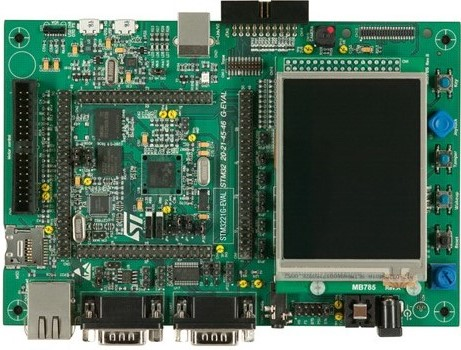
\includegraphics[width = \textwidth]{stm3221g-eval}
\\Rys. 1. Płytka testowa stm3221g-eval
\end{center}


\section{Struktura katalogów w projekcie}

Struktura katalogów w projekcie jest następująca 
\begin{itemize}
\item{ldscript}
\item{libs}
\begin{itemize}
\item{Drivers}
\begin{itemize}
\item{CMSIS}
\item{STM32F2\_HAL\_Driver}
\end{itemize}
\item{wolfssl-3.9.10}
\end{itemize}
\item{misc}
\item{test\_vectors}
\item{workspace}
\begin{itemize}
\item{src}
\item{inc}
\item{build}
\end{itemize}
\end{itemize}

W folderze ldscripts znajdują się skrypty linkera. To one definiują m.in. ile pamięci RAM/flash jest dostępne w procesorze oraz definiują podział pamięci na stertę i stos.\\
W folderze libs, podkatalogu Drivers znajdują się dwie bilioteki procesora STM32F2. Stanowią one swoisty interfejs do części hardwerowej procesora. Pozwalają na zarządzanie np. tatktowania zegarem procesora, konfiguracją timerów, obsługą krpytoprocesorów (badany procesor ma specjalnie dedykowane kryptojednostki wykonujące niektóre algorytmy np. AES, SHA-1) czy portów GPIO.\\
W folderze libs, podkatalogu wolfssl-3.9.10 znajdują się pliki źródłowe badanej biblioteki wolfSSL oraz zbudowana biblioteka.\\
W folderze misc znajdują się różne pliki, które nie mają swoich predefiniowanych katalogów. Są tam pliki opisujące sposób biblioteki wolfSSL, czy konfiguracji połączenia między komputerem klasy PC, a płytką testową z mikrokontrolerem STM32.\\
Folder test\_vectors zawiera dane testowe, które służą do badania wydajnośći poszczególnych implementacji algorytmów. Dzięki wspólnym danym wejściowym, wyniki mogą być bezpośrednio porównywane.\\
W Folderze workspace, w poczególnych podkatalogach znajdują się pliki źródłowe z moją własną implementacją poszczególnych algorytmów, pliki nagłówkowe, a w katalogu pliki powstające w momencie budowania całego projektu (pliki obiektowe oraz plik ELF, który jest wgrywany do procesora).
\section{Instalowanie IDE do programowania STM32}

W pracy zdecydowano się użyć toolchain'u dedykowanego do STM32 dla aplikacji bare metalowych (bez nadrzędnego systemu operacyjnego) GNU ARM Embedded Toolchain. Posiada on kompilator arm-gcc-none-eabi, który wspiera kompilację na większość platform z rodzin Cortex-M i Cortex-R, w szczególności na interesujący nas Cortex-M7. Posiada też wbudowany debugger GDB (GNU Debugger), który pozwala podejrzeć co dzieje się wewnątrz programu (aktualne wartości zmiennych, rejestrów procesora, adresów w pamięci, licznik programu) oraz pozwala na sterowanie jego przebiegiem przez zatrzymywanie cyklu programu w kluczowych momentach przez brakepointy, czy przechodzenie ,,krok po kroku'' między instrukjami.\\
Do zarządzania procesem budowania został użyty program make. Pozwala on na łatwe ustawianie reguł w jaki sposób należy budować poszczególne pliki, ustawia ścieżki do dołączania plików, czy wybór wersji biblioteki z której chcemy korzystać. Dzięki dobremu plikowi Makefile można posiadać wiele konfiguracji do budowania programu i wybierać odpowiednią za pomocą opcji wywołania programu make np. \textit{make all LIBRARY=wolfssl\_no\_hardwarecrypto }

Do wgrywania zbudowanego program został użyty programator SEGGER, który jest już wbudowany w płytkę testową.

Ostantim używanym programem jest OpenOCD (Open On Chip Debugger). Za pomocą interfejsu JTAG dostępnego na płytce komunikuje się on z procesorem, umożliwia semihosting czyli przekazywanie danych z/do komputera w czasie pracy mikroprocesora.

\section{Kompilowanie biblioteki}

Pierwszym krokiem do zbudowania biblioteki jest wybór platformy, na której kod będzie wykonywany. W tym celu edytujemy plik \textit{settings.h} znajdujące się w katalogu \textit{wolfssl-3.9.10/wolfssl/wolfcrypt/}. Ponieważ naszą platformą jest STM32F2, to w pliku odkomentowujemy \#define WOLFSSL\_STM32F2 (linia 92). W późniejszej fazie pracy z biblioteką, okazało się że w pliku trzeba też usunąć \#define KEIL\_INTRINSICS (linia 766). WolfSSL w wersji 3.9.10 jawnie zakłada, że jedynym kompilatorem służącym do zbudowania biblioteki jest płatny kompilator Keil'a. Po usunięciu tej instrukcji dodającej funkcje kompilatora Keil, biblioteka kompiluje się również przy użyciu arm-gcc-none-eabi oraz dowolnych innych kompilatorów języka C na platformę STM32F2.
W celu dalszej konfiguracji biblioteki powstał następujący skrypt bashowy:\\
\texttt{
CC=/c/GNU\_Tools\_ARM\_Embedded/4.9\_2015q3/bin/arm-none-eabi-gcc\\
AR=/c/GNU\_Tools\_ARM\_Embedded/4.9\_2015q3/bin/arm-none-eabi-ar\\
RANLIB=/c/GNU\_Tools\_ARM\_Embedded/4.9\_2015q3/arm-none-eabi/bin/ranlib\\
LDFLAGS=" -lc -specs=nosys.specs"\\
CFLAGS="-mcpu=cortex-m3 -march=armv7-m -mthumb -mlittle-endian -DNO\_WRITEV -DWOLFSSL\_USER\_IO -DWOLFCRYPT\_ONLY\\-I/Drivers/CMSIS/Include\\-I/Drivers/CMSIS/Device/ST/STM32F2xx/Include\\-I/Drivers/STM32F2xx\_StdPeriph\_Lib\_V1.1.0/Libraries/STM32F2xx\_StdPeriph\_Driver/src\\-I/Drivers/STM32F2xx\_HAL\_Driver/Inc \\-I/Drivers/STM32F2xx\_HAL\_Driver/Src\\-I/Drivers/STM32F2xx\_StdPeriph\_Lib\_V1.1.0/Libraries/STM32F2xx\_StdPeriph\_Driver/inc"\\
./configure --host=arm-none-eabi CC=\$CC AR=\$AR RANLIB=\$RANLIB LDFLAGS="\$LDFLAGS" CFLAGS="\$CFLAGS"	
}
\\Zmienna CC przechowuje ścieżkę do kompilatora arm-none-eabi-gcc
\\Zmienna AR przechowuje ścieżkę do programu ar, służącego do tworzenia/modyfikowania/wyciągania danych z archiwum
\\Zmienna RANLIB przechowuje ścieżkę do programu ranlib, który tworzy indeksowaną listę symboli w archiwum
\\Zmienna LDFLAGS zawiera dodatkowe flagi dla linkera. Flaga -lc dodaje bibliotekę libc.a do kompilacji, flaga -specs=nosys.specs oznacza, że aplikacja będzie działała na platformie bez systemu operacyjnego i funkcje systemowe jak np. malloc muszą być dodane przez kompilator
\\Zmienna CFLAGS zawiera dodatkowe zmienne dla kompilatora. Zmienna -mcpu=cortex-m3 oznacza że program będzie wykonywany na platformie Cortex-M3, -march=armv7-m określa architekturę procesora jako ARMv7-M, -mthumb dodaje rozszerzony zestaw instrukcji asemblerowych Thumb, -mlittle-endian oznacza że zmienne w procesorze są pzechowywane w formacie little endian (najmniej znaczący bit jest najmłodszy). Flagi -NO\_WRITEV -WOLFSSL\_USER\_IO oznaczają, że w systemie nie ma żadnych instrukcji wejścia/wyjścia, a użytkownik posiada swoje funkcje IO (eng. input/output). Kolejne flagi zaczynające się od I/ zawierają ścieżki do plików nagłóWkowych i żródłowych bibliotek STM32F2.
\\Ostatnia linia skryptu wywołuje inny skrypt dostarczany przez WolfSSL, który przetwarza wszystkie dane i tworzy własny plik Makefile.
Tak przygotowany plik jest do kompilacji. Poleceniem \textit{make src/libwolfssl.la} kompilujemy bibliotekę do pliku libwolfssl.la. 

\chapter{Pomiar czasu}
Pomiar czasu można wykonać na dwa podstawowe sposoby: przez zastosowanie portów GPIO, lub przez użycie wewnętrznych timerów procesora. Pierwszy sposób zakłada zmianę stanu napięcia w chwilach rozpoczęcia i zakończenia wykonywania algorytmu, a następnie dzięki podpięciu oscyloskopu pomiar częstotliwości zmian napięcia na wybranym pinie. Drugi sposób wykorzystuje timery procesora, który jest w stanie zliczać impulsy z częstotliwością równą częstotliwości taktowania procesora, czyli 96 MHz. W pracy zdecydowano się na drugi sposób z uwagi na łatwiejszą konfigurację projektu oraz pełną automatyzację wykonywania pomiarów.\\
\begin{center}
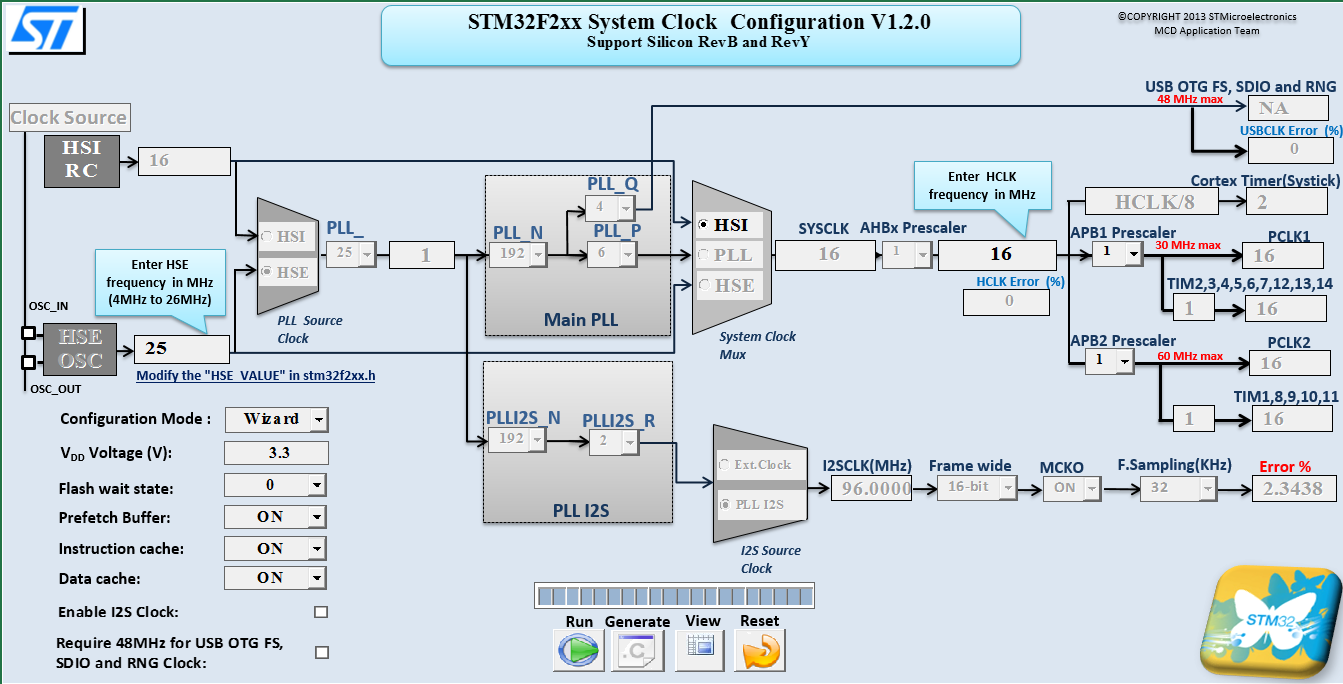
\includegraphics[width = \textwidth]{liczniki}
\\Rys. 2. Schemat konfiguracji licznika
\end{center}

Konfiguracja wewnętrznych timerów została przeprowadzona za pomocą biblioteki HAL. Został wybrany 32-bitowy licznik zliczający przejścia zegara procesora z logicznego ,,0'' na ,,1''. W ten sposób uzyskany został pomiar z dokładnością do $\frac{1}{48000000}$ sekundy i maksymalną mierzoną wartością $2^{32} * \frac{1}{48000000} \approx$ 90 sekund. Do pomiaru czasu służą 3 proste funkcje: inicjalizująca timer, rozpoczynająca oraz kończąca pomiar.
\\Funkcja inicjująca najpierw wybiera timer2 (32-bitowy), ustawia preskaler oraz dzielnik częstotliwości na 1 aby osiągnąć maksymalną dokładność pomiaru oraz ustawia kierunek zliczania impulsów w górę i makysmalną wartość timera na 0xFFFFFFFF:\\
\texttt{
void TimerInit( TIM\_HandleTypeDef *timerHandle)\\
\{\\
\hspace*{10mm}timerHandle->Instance = TIM2;\\
\hspace*{10mm}\_\_TIM2\_CLK\_ENABLE();\\
\hspace*{10mm}timerHandle->Init.Prescaler = 1;\\
\hspace*{10mm}timerHandle->Init.CounterMode = TIM\_COUNTERMODE\_UP;\\
\hspace*{10mm}timerHandle->Init.Period = 0xFFFFFFFF;\\
\hspace*{10mm}timerHandle->Init.ClockDivision = 1;\\\}\\
}
\\Funkcja rozpoczynająca pomiar, wołana po inicjacji timera ustawia aktualną wartość zliczany impulsów:\\
\texttt{
void TimerStart(TIM\_HandleTypeDef *timerHandle)\\
\{\\
\hspace*{10mm}timerHandle->Instance->CNT = 0;\\
\}\\
}
\\Funkcja kończąca pomiar, wołana po inicjacji timera odczytuje aktualną ilość zliczonych impulsów i zwraca jej wartość:\\
\texttt{
uint32\_t TimerStop(TIM\_HandleTypeDef *timerHandle)\\
\{\\
\hspace*{10mm}return timerHandle->Instance->CNT;\\
\}
}
\section{Wyniki dla SHA1}
Przykładowe wyniki pomiarów dla 30 wykonań algorytmu SHA-1 wyglądają następująco:
\begin{center}

\begin{tabular}{|c|c|c|c|c|c|c|c|}
\hline 
\multicolumn{4}{|c|}{Software crypto} & \multicolumn{4}{|c|}{hadware crypto} \\
\hline 
\multicolumn{2}{|c|}{32 bajty} & \multicolumn{2}{|c|}{64 bajty} & \multicolumn{2}{|c|}{32 bajty} & \multicolumn{2}{|c|}{64 bajty} \\
\hline 
licznik & czas[ms] & licznik & czas[ms] & licznik & czas[ms] & licznik & czas[ms] \\
\hline 
690 &	0.014 &	1261 &	0.026 &	253 &	0.005 &	318 &	0.007 \\
690 &	0.014 &	1262 &	0.026 &	252 &	0.005 &	317 &	0.007 \\
690 &	0.014 &	1260 &	0.026 &	253 &	0.005 &	318 &	0.007 \\
690 &	0.014 &	1260 &	0.026 &	253 &	0.005 &	318 &	0.007 \\
690 &	0.014 &	1260 &	0.026 &	253 &	0.005 &	318 &	0.007 \\
690 &	0.014 &	1261 &	0.026 &	253 &	0.005 &	317 &	0.007 \\
690 &	0.014 &	1260 &	0.026 &	253 &	0.005 &	318 &	0.007 \\
690 &	0.014 &	1260 &	0.026 &	253 &	0.005 &	317 &	0.007 \\
690 &	0.014 &	1260 &	0.026 &	252 &	0.005 &	318 &	0.007 \\
690 &	0.014 &	1260 &	0.026 &	253 &	0.005 &	317 &	0.007 \\
692 &	0.014 &	1261 &	0.026 &	253 &	0.005 &	318 &	0.007 \\
690 &	0.014 &	1260 &	0.026 &	253 &	0.005 &	318 &	0.007 \\
690 &	0.014 &	1260 &	0.026 &	253 &	0.005 &	318 &	0.007 \\
690 &	0.014 &	1261 &	0.026 &	252 &	0.005 &	318 &	0.007 \\
691 &	0.014 &	1260 &	0.026 &	253 &	0.005 &	317 &	0.007 \\
691 &	0.014 &	1260 &	0.026 &	253 &	0.005 &	317 &	0.007 \\
690 &	0.014 &	1260 &	0.026 &	253 &	0.005 &	317 &	0.007 \\
690 &	0.014 &	1260 &	0.026 &	253 &	0.005 &	317 &	0.007 \\
690 &	0.014 &	1270 &	0.026 &	252 &	0.005 &	317 &	0.007 \\
690 &	0.014 &	1260 &	0.026 &	252 &	0.005 &	317 &	0.007 \\
690 &	0.014 &	1260 &	0.026 &	253 &	0.005 &	318 &	0.007 \\
690 &	0.014 &	1260 &	0.026 &	253 &	0.005 &	317 &	0.007 \\
690 &	0.014 &	1260 &	0.026 &	253 &	0.005 &	318 &	0.007 \\
690 &	0.014 &	1261 &	0.026 &	252 &	0.005 &	318 &	0.007 \\
690 &	0.014 &	1261 &	0.026 &	253 &	0.005 &	317 &	0.007 \\
690 &	0.014 &	1260 &	0.026 &	253 &	0.005 &	318 &	0.007 \\
690 &	0.014 &	1261 &	0.026 &	253 &	0.005 &	318 &	0.007 \\
690 &	0.014 &	1260 &	0.026 &	253 &	0.005 &	317 &	0.007 \\
690 &	0.014 &	1260 &	0.026 &	253 &	0.005 &	317 &	0.007 \\
690 &	0.014 &	1261 &	0.026 &	253 &	0.005 &	318 &	0.007 \\

\hline 
\end{tabular} 

\end{center}
\chapter{Biblioteka WolfSSL}
WolfSSL to opensourcowa biblioteka kryptograficzna napisana w języku C. Jest przeznaczona przede wszystkim na systemy wbudowane ze względu na mały rozmiar, wysoką prędkość biblioteki, oraz optymalizację na wiele platform embedded na czele z STM32, freescalem czy Texas Instrument. W bibliotece znajduje się silnik kryptograficzny wolfcrypt, który został poddany badaniom. W celu pobrania kodów źródłowych biblioteki wchodzimy na stronę producenta: www.wolfssl.com i pobieramy bibliotekę w najnowszej wersji 3.9.10

\chapter{AES}
Quisque nibh sapien, lobortis posuere, dignissim id, ultricies ut,
est. Cras nec nunc nec ligula placerat ullamcorper. Maecenas consequat
consequat nisi. Etiam varius. Vestibulum ante ipsum primis in faucibus
orci luctus et ultrices posuere cubilia Curae; Ut risus velit,
vulputate aliquet, tristique nec, ullamcorper et, justo. In hac
habitasse platea dictumst. Suspendisse rhoncus venenatis eros. Proin
nec lorem nec sem auctor lobortis. Quisque ac dolor. Suspendisse
potenti. Maecenas fermentum sem non neque. Cras nonummy commodo
libero. Sed in erat.


\section{Software}
Nulla quis enim ut erat rutrum feugiat. Suspendisse lacinia tempor
mi. Vestibulum nec lacus sed est rutrum cursus. Cras ultrices est eget
pede. Sed ullamcorper ultrices tellus. Nulla lectus. Nunc
consectetuer, quam quis sagittis vulputate, dui leo molestie augue, a
commodo tellus tortor a turpis. Nam et ipsum. Ut placerat aliquet
enim. Suspendisse potenti. Etiam volutpat tortor in mauris. Praesent
dapibus congue arcu.

\section{Hardware}
Aliquam quis sem. Phasellus tincidunt fringilla metus. Sed id
purus. Ut consectetuer urna nec sapien. Sed sed odio sed lectus
imperdiet ultricies. Suspendisse semper congue pede. Etiam facilisis
sapien nec dolor. Pellentesque sodales rutrum lorem. Aliquam tristique
diam ac lacus. Vestibulum ante ipsum primis in faucibus orci luctus et
ultrices posuere cubilia Curae; Duis sit amet pede. Suspendisse ut
dui. Aliquam massa quam, facilisis in, vulputate non, imperdiet quis,
diam. Nullam feugiat. Morbi non dolor et eros fringilla
gravida. Pellentesque rhoncus, odio ac fringilla varius, ante nunc
hendrerit massa, sed varius est est eu massa.


\begin{itemize}
\item Mauris nonummy lorem at orci.
\item Donec accumsan aliquam libero.
\item Donec fringilla ultricies diam.
\item Nulla venenatis est non ligula.
\item Morbi in mi convallis dolor accumsan egestas.
\item Sed euismod nibh in nulla.
\item Sed rhoncus lorem at lectus.
\item Pellentesque fermentum rutrum dui.
\end{itemize}

Proin euismod. Curabitur adipiscing ipsum ac augue. Maecenas hendrerit
tortor non velit suscipit laoreet. Aenean tempus. Nunc
convallis. Aenean sed erat. Etiam massa nulla, interdum pretium,
faucibus nec, sollicitudin vitae, lorem. Quisque vulputate cursus
pede. Phasellus enim ipsum, lacinia vel, sodales ac, faucibus et,
tortor. Aliquam hendrerit. Aliquam erat volutpat. Quisque dui lorem,
placerat eu, commodo et, condimentum sed, nibh. Nulla eu orci in nibh
pretium tincidunt. Pellentesque mi massa, fringilla eu, vehicula
consectetuer, sodales a, nisi.


\chapter{DES}
Nulla a nisl at nisl dignissim facilisis. In sit amet mi. Nunc
ullamcorper, ligula vel aliquam pretium, nulla mauris euismod ipsum,
sit amet tempus massa nulla non elit. Donec congue. Nulla
purus. Aenean dui orci, ornare quis, interdum sed, molestie ac,
tellus. Lorem ipsum dolor sit amet, consectetuer adipiscing
elit. Quisque mollis diam nec elit. Maecenas nec enim. Maecenas
facilisis urna quis arcu. Fusce posuere.


\appendix
\chapter{SHA}
Donec cursus nulla vitae pede. Etiam quam pede, aliquet ut,
pellentesque sed, sagittis non, est. Quisque egestas malesuada
risus. Maecenas ultricies libero a quam. Nullam feugiat arcu. Class
aptent taciti sociosqu ad litora torquent per conubia nostra, per
inceptos hymenaeos. In interdum, risus ut gravida sollicitudin, leo
sapien commodo dui, non consectetuer nisl nunc ac massa. Mauris a orci
in eros venenatis euismod. Curabitur orci. Quisque pharetra, dui sed
dignissim hendrerit, nibh ante malesuada eros, sed tincidunt magna
lorem a tellus. Aliquam erat volutpat. Aenean pulvinar, metus et
mattis dictum, massa lacus semper purus, quis vehicula augue mi et
leo. Ut eu ipsum. Sed dictum dapibus nisi. Cras mattis. Nulla sed
augue ac sem tempus condimentum.

\chapter{SHA-256}
Donec cursus nulla vitae pede. Etiam quam pede, aliquet ut,
pellentesque sed, sagittis non, est. Quisque egestas malesuada
risus. Maecenas ultricies libero a quam. Nullam feugiat arcu. Class
aptent taciti sociosqu ad litora torquent per conubia nostra, per
inceptos hymenaeos. In interdum, risus ut gravida sollicitudin, leo
sapien commodo dui, non consectetuer nisl nunc ac massa. Mauris a orci
in eros venenatis euismod. Curabitur orci. Quisque pharetra, dui sed
dignissim hendrerit, nibh ante malesuada eros, sed tincidunt magna
lorem a tellus. Aliquam erat volutpat. Aenean pulvinar, metus et
mattis dictum, massa lacus semper purus, quis vehicula augue mi et
leo. Ut eu ipsum. Sed dictum dapibus nisi. Cras mattis. Nulla sed
augue ac sem tempus condimentum.


\addcontentsline{toc}{chapter}{Bibliografia} %utworzenie w
                                             %spisietreści pozycji
                                             %Bibliografia

\bibliography{bibliografia} % wstawia bibliografię korzystając z pliku
                            % bibliografia.bib - dotyczy BibTeXa,
                            % jeĚźeli nie korzystamy z BibTeXa naleĚźy
                            % użyć otoczenia thebibliography

%opcjonalnie może się tu pojawić spis rysunków i tabel
% \listoffigures
% \listoftables
\end{document}

